\documentclass[12pt]{report}
\usepackage[a4paper, margin=1in]{geometry}
\usepackage{graphicx}
\usepackage{amsmath}
\usepackage{url}
\usepackage[hidelinks]{hyperref}
\usepackage{caption}
\usepackage{subcaption}
\usepackage{natbib}
\usepackage{array}
\usepackage{booktabs}
\usepackage{multirow}
\usepackage[table]{xcolor}
\usepackage{pgfgantt}
\usepackage{enumitem}





\usepackage{setspace}
\onehalfspacing

\title{%
    \vspace{-4cm} % Space above title
    Fed-MStacking: Heterogeneous Federated Learning With Stacking \\ 
    Misaligned Labels for Abnormal Heart Sound Detection \\
    \vspace{0.5cm} % Space below title
}
\author{%
    Temidayo Tom Afelumo \\
    \vspace{0.2cm} % Space after name
    \large{Registration: 2411655} \\
    \vspace{0.5cm} % Space before supervisor
    % Supervisor: Dr. \\
    \vspace{5cm} % Space after supervisor
    School of Computer Science \& Electronic Engineering \\
    University of Essex \\
    \vspace{0.5cm} % Space at bottom
}
\date{\vspace{6cm}\ July 2, 2025} % Space before date

\begin{document}

\maketitle




\begin{abstract}
    Cardiovascular diseases (CVDs) are the world's leading cause of death, with early diagnosis often limited in low-resource settings by inconsistent manual interpretation and privacy concerns around centralized AI solutions. This project proposes \textbf{MStacking}, a novel federated learning (FL) framework designed to detect abnormal heart sounds while safeguarding patient data. In MStacking, each healthcare institution trains its own binary classifier using only local data—typically covering the normal class and one abnormal class—reflecting real-world disadvantages such as label imbalance and varied computing resources.
    
    Instead of sharing sensitive data or model parameters, clients send prediction scores and data density estimates to a central server. A meta-learner then combines these outputs using a stacking ensemble approach to build a comprehensive global classifier. The development supports multimodal inputs, including 1D acoustic signals and 2D spectrograms of phonocardiogram (PCG) recordings.
    
    Experiments using publicly available datasets, like PhysioNet/CinC 2016, simulate federated conditions to benchmark MStacking against traditional centralized and FL models. Key evaluation metrics include accuracy, communication efficiency, and robustness to label noise and data imbalance.
    
    By enabling collaborative model training without exposing patient data, MStacking offers a practical, scalable, and privacy-preserving solution for AI-powered auscultation—especially in decentralized and diverse healthcare environments.
    \end{abstract}
    
    

\tableofcontents
\listoffigures
\listoftables

\newpage
\chapter{Introduction}

Cardiovascular diseases (CVDs) remain the leading cause of illness and death globally, with the burden falling especially hard on people in low- and middle-income countries. In many of these settings, access to advanced diagnostic tools like ECGs and cardiac imaging is limited \cite{roth2020global}. In contrast, listening to heart sounds—a method known as auscultation—offers a non-invasive, affordable, and widely accessible way to detect heart conditions such as valve disorders, coronary artery disease, and arrhythmias \cite{li2020review, roy2019heart}.

Thanks to recent advances in artificial intelligence (AI) and the growing ecosystem of the Internet of Health Things (IoHT), it’s now possible to automate and remotely monitor these heart sounds. This development opens the door to early diagnosis and continuous care, even in remote or resource-limited clinics \cite{winther2021advanced, qian2019deep}. However, most existing AI models rely on centralized data collection, which poses serious privacy risks and faces ethical and legal constraints, especially under regulations like HIPAA \cite{swarup2018digital}. This makes many hospitals hesitant to share sensitive patient data.

Federated Learning (FL) offers a promising alternative. It allows institutions to collaboratively train models without ever exchanging raw data \cite{xu2021federated}. Still, traditional FL methods often assume all participants use the same model types and share the same label distributions—an assumption that doesn’t reflect reality. Clinics may only have access to a narrow slice of heart sound data and might use different machine learning tools based on their resources \cite{qian2021artificial,qian2021can}.

To tackle these limitations, we introduce \textbf{MStacking}—a federated learning framework that supports heterogeneous models and learns from partially labeled datasets. It uses a stacking ensemble method to merge insights from each client’s locally trained model, combining both raw acoustic features and time–frequency images like PCG spectrograms. MStacking aims to make AI-assisted auscultation truly practical and inclusive, supporting scalable and privacy-preserving diagnostics across diverse medical environments \cite{xu2021federated}.


\chapter{Literature Review}

\section{Abnormal Heart Sound Detection}

% Cardiovascular diseases (CVDs) continue to be the top cause of death worldwide, making early diagnosis a critical step in saving lives and improving quality of care. While advanced tools like echocardiograms and ECGs are commonly available in high-income countries, many low- and middle-income regions lack the resources to access these technologies. In such contexts, heart auscultation—the practice of listening to heart sounds using a stethoscope—offers a practical, non-invasive, and affordable way to screen for abnormalities like murmurs, valve disorders, and arrhythmias. However, the reliability of auscultation depends greatly on the experience and skill of the clinician, leading to inconsistencies and potential diagnostic errors.

% To address this, the field has seen significant progress with computer-aided auscultation (CAA) systems. These tools pair digital stethoscopes with signal processing and machine learning techniques to automate and standardize heart sound analysis \cite{swarup2018digital}. They extract key features from phonocardiogram (PCG) recordings—such as energy, entropy, time-frequency patterns, and wavelet coefficients—to identify components like the first (S1) and second (S2) heart sounds, as well as murmurs and abnormal extra sounds \cite{li2020review, qian2019deep}. Traditional machine learning models, including support vector machines (SVMs), decision trees, and random forests, have shown promising results, particularly when trained on curated datasets.

% With the emergence of deep learning, more sophisticated models like convolutional neural networks (CNNs) and recurrent neural networks (RNNs) have been used to capture intricate patterns directly from raw or preprocessed PCG signals \cite{winther2021advanced, clifford2016classification}. Many recent approaches combine both 1D audio signals and 2D visual representations—such as spectrograms—to leverage complementary information and boost classification accuracy. Public datasets like the PhysioNet/CinC 2016 Challenge have played a key role by offering a wide range of expert-labeled PCG recordings for training and evaluation \cite{clifford2016classification, liu2016openaccess}.

Cardiovascular diseases (CVDs) remain the leading cause of mortality globally, emphasizing the need for early and accurate diagnosis to improve patient outcomes and quality of care. While diagnostic tools such as echocardiograms and electrocardiograms (ECGs) are standard in high-income countries, many low- and middle-income regions face significant challenges in accessing these technologies. In such settings, heart auscultation—the practice of listening to heart sounds using a stethoscope—serves as a practical, non-invasive, and affordable screening method for detecting abnormalities like murmurs, valve disorders, and arrhythmias. However, the effectiveness of auscultation heavily relies on the clinician's expertise, which can result in inconsistent interpretations and diagnostic errors.

To overcome these limitations, significant progress has been made in computer-aided auscultation (CAA) systems. These systems combine digital stethoscopes with advanced signal processing and machine learning algorithms to enable automated and standardized analysis of heart sounds \cite{swarup2018digital}. CAA systems extract relevant features from phonocardiogram (PCG) signals—such as energy, entropy, time-frequency characteristics, and wavelet transforms—to detect key components like the first (S1) and second (S2) heart sounds, murmurs, and abnormal extra sounds \cite{li2020review, qian2019deep}. Traditional machine learning methods, including support vector machines (SVMs), decision trees, and random forests, have demonstrated strong performance when applied to well-annotated datasets.

The advent of deep learning has further enhanced these capabilities, with models such as convolutional neural networks (CNNs) and recurrent neural networks (RNNs) being utilized to learn complex patterns from raw or preprocessed PCG recordings \cite{winther2021advanced, clifford2016classification}. Modern approaches often integrate both 1D audio waveforms and 2D visual features—like spectrograms—to capture complementary information and improve classification accuracy. The availability of publicly accessible datasets, such as those from the PhysioNet/CinC 2016 Challenge, has greatly facilitated the development and benchmarking of these systems by providing a wide array of expert-labeled heart sound recordings \cite{clifford2016classification, liu2016openaccess}.


\begin{figure}[htbp]
    \centering
    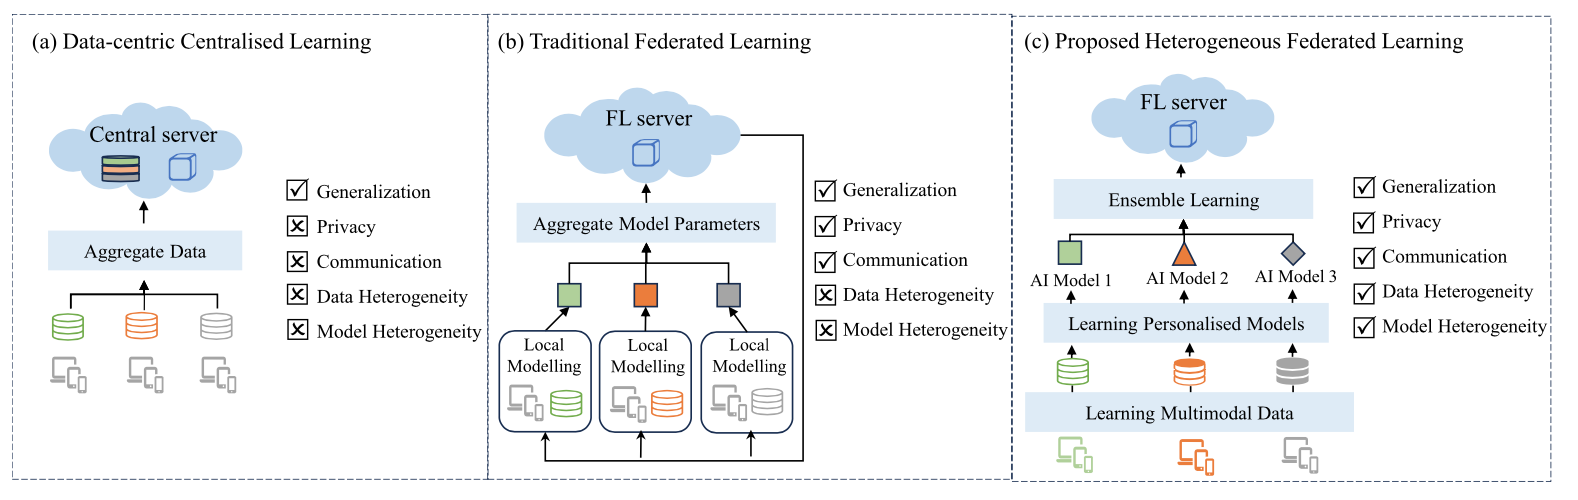
\includegraphics [width=0.9\textwidth]{./Figures/fig.png}
    \caption{Research background. (a) Data-centric centralised learning, which pools data together to train a central ML model. (b) In traditional FL, the global model is trained under the coordination of the central server while data resides in different data silos. (c) The proposed heterogeneous FL, which addresses the limitations of FL through ensemble personalised models learning. 
}
    \label{fig:enter-label}
\end{figure}


Despite major strides in heart sound analysis, several challenges remain. One persistent issue is the variability between patients, which can affect how heart sounds are interpreted. Recordings often contain background noise or artifacts, and some critical heart conditions—like rare anomalies—are underrepresented in datasets, making it harder for models to learn from them. For AI systems to be trusted and adopted in clinical settings, they also need to generalize well across populations, be interpretable by healthcare professionals, and run efficiently on edge devices such as digital stethoscopes or wearables.

To tackle these hurdles, researchers are turning to methods like domain adaptation to help models adapt across different patient groups and clinical conditions. Explainable AI (XAI) techniques are being developed to make model decisions more transparent, helping clinicians understand why a certain prediction was made. Meanwhile, privacy-preserving approaches like federated learning are gaining traction, enabling collaborative model training without sharing sensitive patient data. Together, these innovations are paving the way toward a scalable and equitable future for AI-powered heart sound diagnostics—one that could benefit patients around the world regardless of where they live.

\section{AI and IoHT in Remote Healthcare}

The Internet of Health Things (IoHT) brings together wearable devices, mobile health applications, and smart sensors to enable continuous patient monitoring and real-time data collection. This integrated ecosystem allows healthcare providers to remotely track key physiological signals such as heart rate, respiration, and body temperature—an especially valuable tool for managing chronic conditions and supporting elderly populations \cite{alshamrani2022iot, qian2021artificial}.

Artificial intelligence (AI) takes this a step further by analyzing the large volumes of multimodal data generated by these devices. With AI, systems can detect early warning signs, issue timely alerts, and offer tailored health recommendations—all while reducing the workload on clinicians and giving patients more control over their care \cite{qian2021can}.

However, traditional AI systems typically rely on centralized data collection, where patient information is uploaded to remote servers for model training. While effective, this approach poses significant privacy and security risks. Healthcare data is not only sensitive but also highly regulated, and centralization increases the chance of breaches and biases—especially when the training data doesn’t reflect diverse populations \cite{xu2021federated}.

To overcome these limitations, federated learning has emerged as a powerful alternative. Rather than sharing raw data, federated learning allows models to be trained locally on each device or institution’s data and then aggregated into a shared global model. This preserves privacy, reduces data exposure, and fosters secure collaboration across different healthcare stakeholders—all while maintaining the performance benefits of modern AI.


\section{Federated Learning in Healthcare}
Federated learning (FL) offers a privacy-conscious way for healthcare institutions to collaboratively train AI models without sharing sensitive patient data~\cite{mcmahan2017communication}. Instead of moving data, each institution trains models locally and only shares model updates with a central server. Using algorithms like FedAvg, these updates are combined to build a stronger global model. As shown in Figure~\ref{fig:fl_workflow}, this process supports local training, centralized aggregation, and privacy by design. FL is already proving effective in medical use cases like disease prediction~\cite{xu2021federated}, mortality risk estimation~\cite{huang2019patient}, and secure electronic health record (EHR) sharing~\cite{brisimi2018federated, tramel2019federated}.

\begin{figure}[ht]
    \centering
    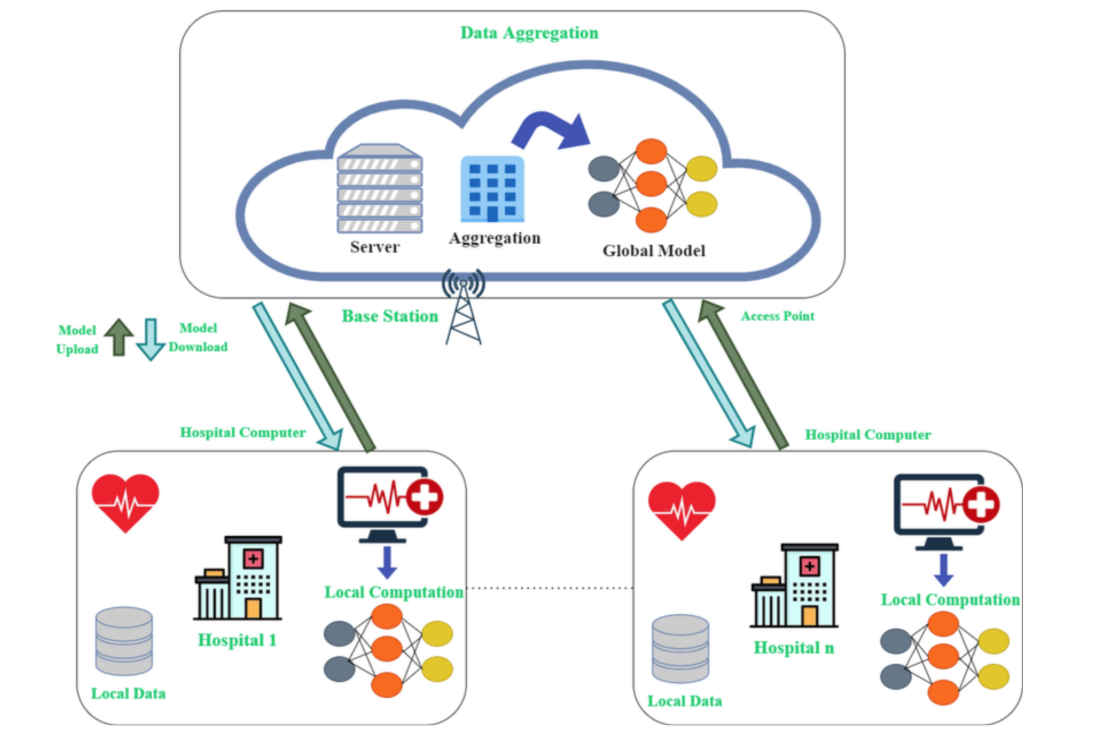
\includegraphics[width=0.9\textwidth]{./Figures/fig2.png}
    \caption{Federated learning workflow with local model training, secure aggregation, and global model distribution.}
    \label{fig:fl_workflow}
\end{figure}

Despite its promise, real-world FL systems face three major challenges, as illustrated in Figure~\ref{fig:fl_workflow}: (1) non-identical data distributions (non-IID) across institutions~\cite{nguyen2022federated}, (2) differences in local model architectures~\cite{yoo2021personalized}, and (3) incomplete class labels within client datasets~\cite{zhang2022federated}. While earlier studies~\cite{qiu2022binary, qiu2024multiclass} have shown FL’s potential for heart sound classification, they often assumed ideal scenarios—uniform models and fully aligned label spaces. For FL to succeed in clinical settings, its architecture must adapt to these real-world constraints.

\section{Personalization and Heterogeneity in FL}
To better reflect the diversity across clients in federated learning, researchers have explored several personalization strategies. These include clustered FL~\cite{yoo2021personalized}, multi-branch architectures~\cite{mori2023multi}, and client-specific training techniques  \cite{tan2023towards} \cite{huang2022learn}. Ensemble and semi-supervised approaches have also shown promise in managing non-IID settings, as seen in studies like~\cite{itahara2023distillation, shaik2022fedstack}. For instance, FedStack~\cite{shaik2022fedstack} used a stacking ensemble for personalized activity monitoring, while Liu et al.~\cite{xu2023federated} tackled inconsistent label distributions in multi-organ segmentation using federated ensembles. Collectively, these efforts highlight the potential of ensemble learning—especially model stacking—as a practical solution to heterogeneity and label misalignment in FL.

\section{Ensemble Learning and Model Stacking}
Ensemble learning techniques like bagging, boosting, and stacking are well-known for enhancing model generalization and robustness~\cite{buhlmann2012ensemble, ribeiro2020ensemble}. Among these, stacking stands out for its ability to combine diverse model architectures, making it particularly valuable in settings like network intrusion detection\cite{zhang2021multi,rajagopal2020stacking} and time-series forecasting~\cite{ribeiro2020ensemble}. In federated learning scenarios, stacking is especially effective because client models often differ in structure due to varying computational capacities or domain-specific needs~\cite{lin2020ensemble}. By training a meta-model on the predictions from these heterogeneous clients, stacking offers a practical way to integrate their outputs—an approach particularly beneficial for complex tasks like multi-class heart sound classification, where clients may have incomplete label sets~\cite{liu2024cybersecurity}.

\section{Summary and Gaps}
While previous research has applied federated learning to medical diagnostics and explored ensemble strategies for model fusion, few have tackled the combined challenges of label misalignment, client model heterogeneity, and multimodal auscultation data. Our proposed framework, \textbf{MStacking}, addresses this gap by using a stacking ensemble approach within a federated learning setup. This allows integration of insights from clients with varying model types and incomplete label spaces—conditions common in real-world healthcare. By doing so, MStacking offers a practical and scalable path toward deploying AI-assisted auscultation across diverse, decentralized medical institutions.

% \end{document}
\chapter{Goals}

\section{Goals}
The primary goal of this project is to develop \textbf{MStacking}, a heterogeneous federated learning framework tailored for classifying abnormal heart sounds in a privacy-preserving manner. The system is designed to function effectively across decentralized healthcare settings, where institutions vary in both computational capabilities and the types of heart sound data they can access. By using a stacking ensemble strategy, MStacking enables collaborative learning without requiring sensitive patient data to be shared, aiming to deliver a more accurate, robust, and adaptable AI-driven auscultation tool.

\section{Objectives}
This project is guided by the following objectives:
\begin{itemize}
    \item \textbf{Support model heterogeneity:} Build a federated system that allows each client to choose its own model architecture based on local data volume and hardware constraints.
    \item \textbf{Stacking ensemble integration:} Use meta-learning to combine predictions from various client models into a unified global classifier, even when local label distributions differ.
    \item \textbf{Leverage multimodal data:} Enhance classification by incorporating both 1D acoustic features and 2D spectrogram representations of phonocardiogram (PCG) signals.
    \item \textbf{Preserve data privacy:} Avoid direct data sharing by transmitting only high-level model outputs and statistical metadata between clients and the central server.
    \item \textbf{Benchmark performance:} Evaluate MStacking against centralized and traditional federated learning methods using public datasets, with a focus on accuracy, generalization, and resilience to real-world data challenges.
\end{itemize}

\section{Scope and Limitations}
\subsection*{Scope}
This project centers on building a proof-of-concept federated learning framework—MStacking—for classifying abnormal heart sounds using heterogeneous client models and misaligned class labels. The system is tested in a simulated federated environment using public datasets like the PhysioNet/CinC 2016 Challenge and other open-access PCG sources. It supports multimodal input types, such as 1D audio signals and 2D spectrograms, and accommodates various model architectures (e.g., CNNs, random forests, FNNs) chosen by individual clients. Development is based on open-source libraries (e.g., PyTorch, Flower/FedML), with training designed to mimic privacy-preserving, decentralized healthcare scenarios.

\subsection*{Limitations}
\begin{itemize}
    \item The prototype is simulation-only; it won’t be deployed in real hospitals or connected to physical stethoscope devices.
    \item Experiments use static, publicly available datasets and do not involve real-time or clinical data.
    \item Due to time and resource constraints, extensive hyperparameter tuning and in-depth ablation analysis are outside the project scope.
    \item The focus is solely on classification tasks—regression or diagnostic recommendation features are not included.
    \item Evaluation relies on offline performance metrics (e.g., accuracy, F1-score), without clinical trials or human-in-the-loop validation.
\end{itemize}

\chapter{Methodology}
\section{Overview of the Proposed System}


This project introduces \textbf{MStacking}, a novel heterogeneous federated learning (FL) framework for classifying abnormal heart sounds from decentralized, privacy-sensitive data. The key challenge addressed is that hospitals often use different machine learning models suited to their data and computing capabilities, and typically only have access to a subset of heart sound classes—leading to label misalignment.

To solve this, MStacking employs a stacking ensemble strategy. Each hospital (client) trains a binary classifier using its local data—usually covering one abnormal class and the normal class—and sends prediction scores and density estimations (not raw data) to a central server. There, a meta-learner integrates these diverse outputs into a unified, global multi-class model, enabling collaborative learning without compromising patient privacy.

A summary of prominent studies utilizing the PhysioNet/CinC 2016 dataset is presented in Table~\ref{tab:physionet_summary}, highlighting the evolution of machine learning applications in heart sound classification.

\begin{table}[h]
\centering
\caption{Summary of Studies Using the PhysioNet/CinC Challenge 2016}
\label{tab:physionet_summary}
\begin{tabular}{|p{3.5cm}|p{1.5cm}|p{3.5cm}|p{3cm}|p{4cm}|}
\hline
\textbf{Study} & \textbf{Year} & \textbf{Task} & \textbf{Model(s) Used} & \textbf{Contribution} \\
\hline
\cite{clifford2016classification} & 2016 & Normal/Abnormal Classification & Ensemble SVMs & Introduced the PhysioNet Challenge dataset \\
\hline
\cite{liu2016open} & 2016 & Classifier Evaluation & Open baseline models & Created open-access benchmark for PCG classifiers \\
\hline
\cite{wang2023explainability} & 2023 & Explainability in PCG Detection & SHAP + FNN & Applied feature attribution methods to enhance transparency \\
\hline
\cite{qiu2022fl} & 2022 & FL for Binary Heart Sound Detection & CNN (FedAvg) & Early federated prototype for heart sound classification \\
\hline
Qiu et al. (This Work) & 2024 & Multi-Class FL for PCG Analysis & RF, FNN, CNN (Hetero) & Introduces MStacking with misaligned labels and heterogeneity \\
\hline
\end{tabular}
\end{table}

\section{Local Model Architecture}

\subsection{Local Model Architecture}
\label{sec:local_model_architecture}

In the MStacking setup, each hospital independently chooses and trains a binary classifier tailored to its dataset size, signal type, and computational capacity (see Figure~\ref{fig:local_models}). Three model types are supported:

\begin{itemize}
    \item \textbf{Random Forest (RF)}: Ideal for low-resource clients with structured feature data. RF ensembles decision trees built on bootstrap samples and uses the Gini index for splits.
    
    \item \textbf{Feedforward Neural Network (FNN)}: Suitable for clients with moderate resources and low-dimensional data. FNNs learn non-linear patterns through layers of neurons trained via backpropagation.
    
    \item \textbf{Convolutional Neural Network (CNN)}: Best for institutions handling spectrograms (e.g., from Continuous Wavelet Transform). CNNs use convolutional layers, global adaptive pooling (GAP), and fully connected layers to classify input efficiently.
\end{itemize}

All models are trained using cross-entropy loss and the Adam optimizer. Clients follow a ``star-structured'' label setup—each has the normal class ($y=0$) and one abnormal class ($y=m$), mimicking real-world healthcare data limitations.

\begin{figure}[h]
    \centering
    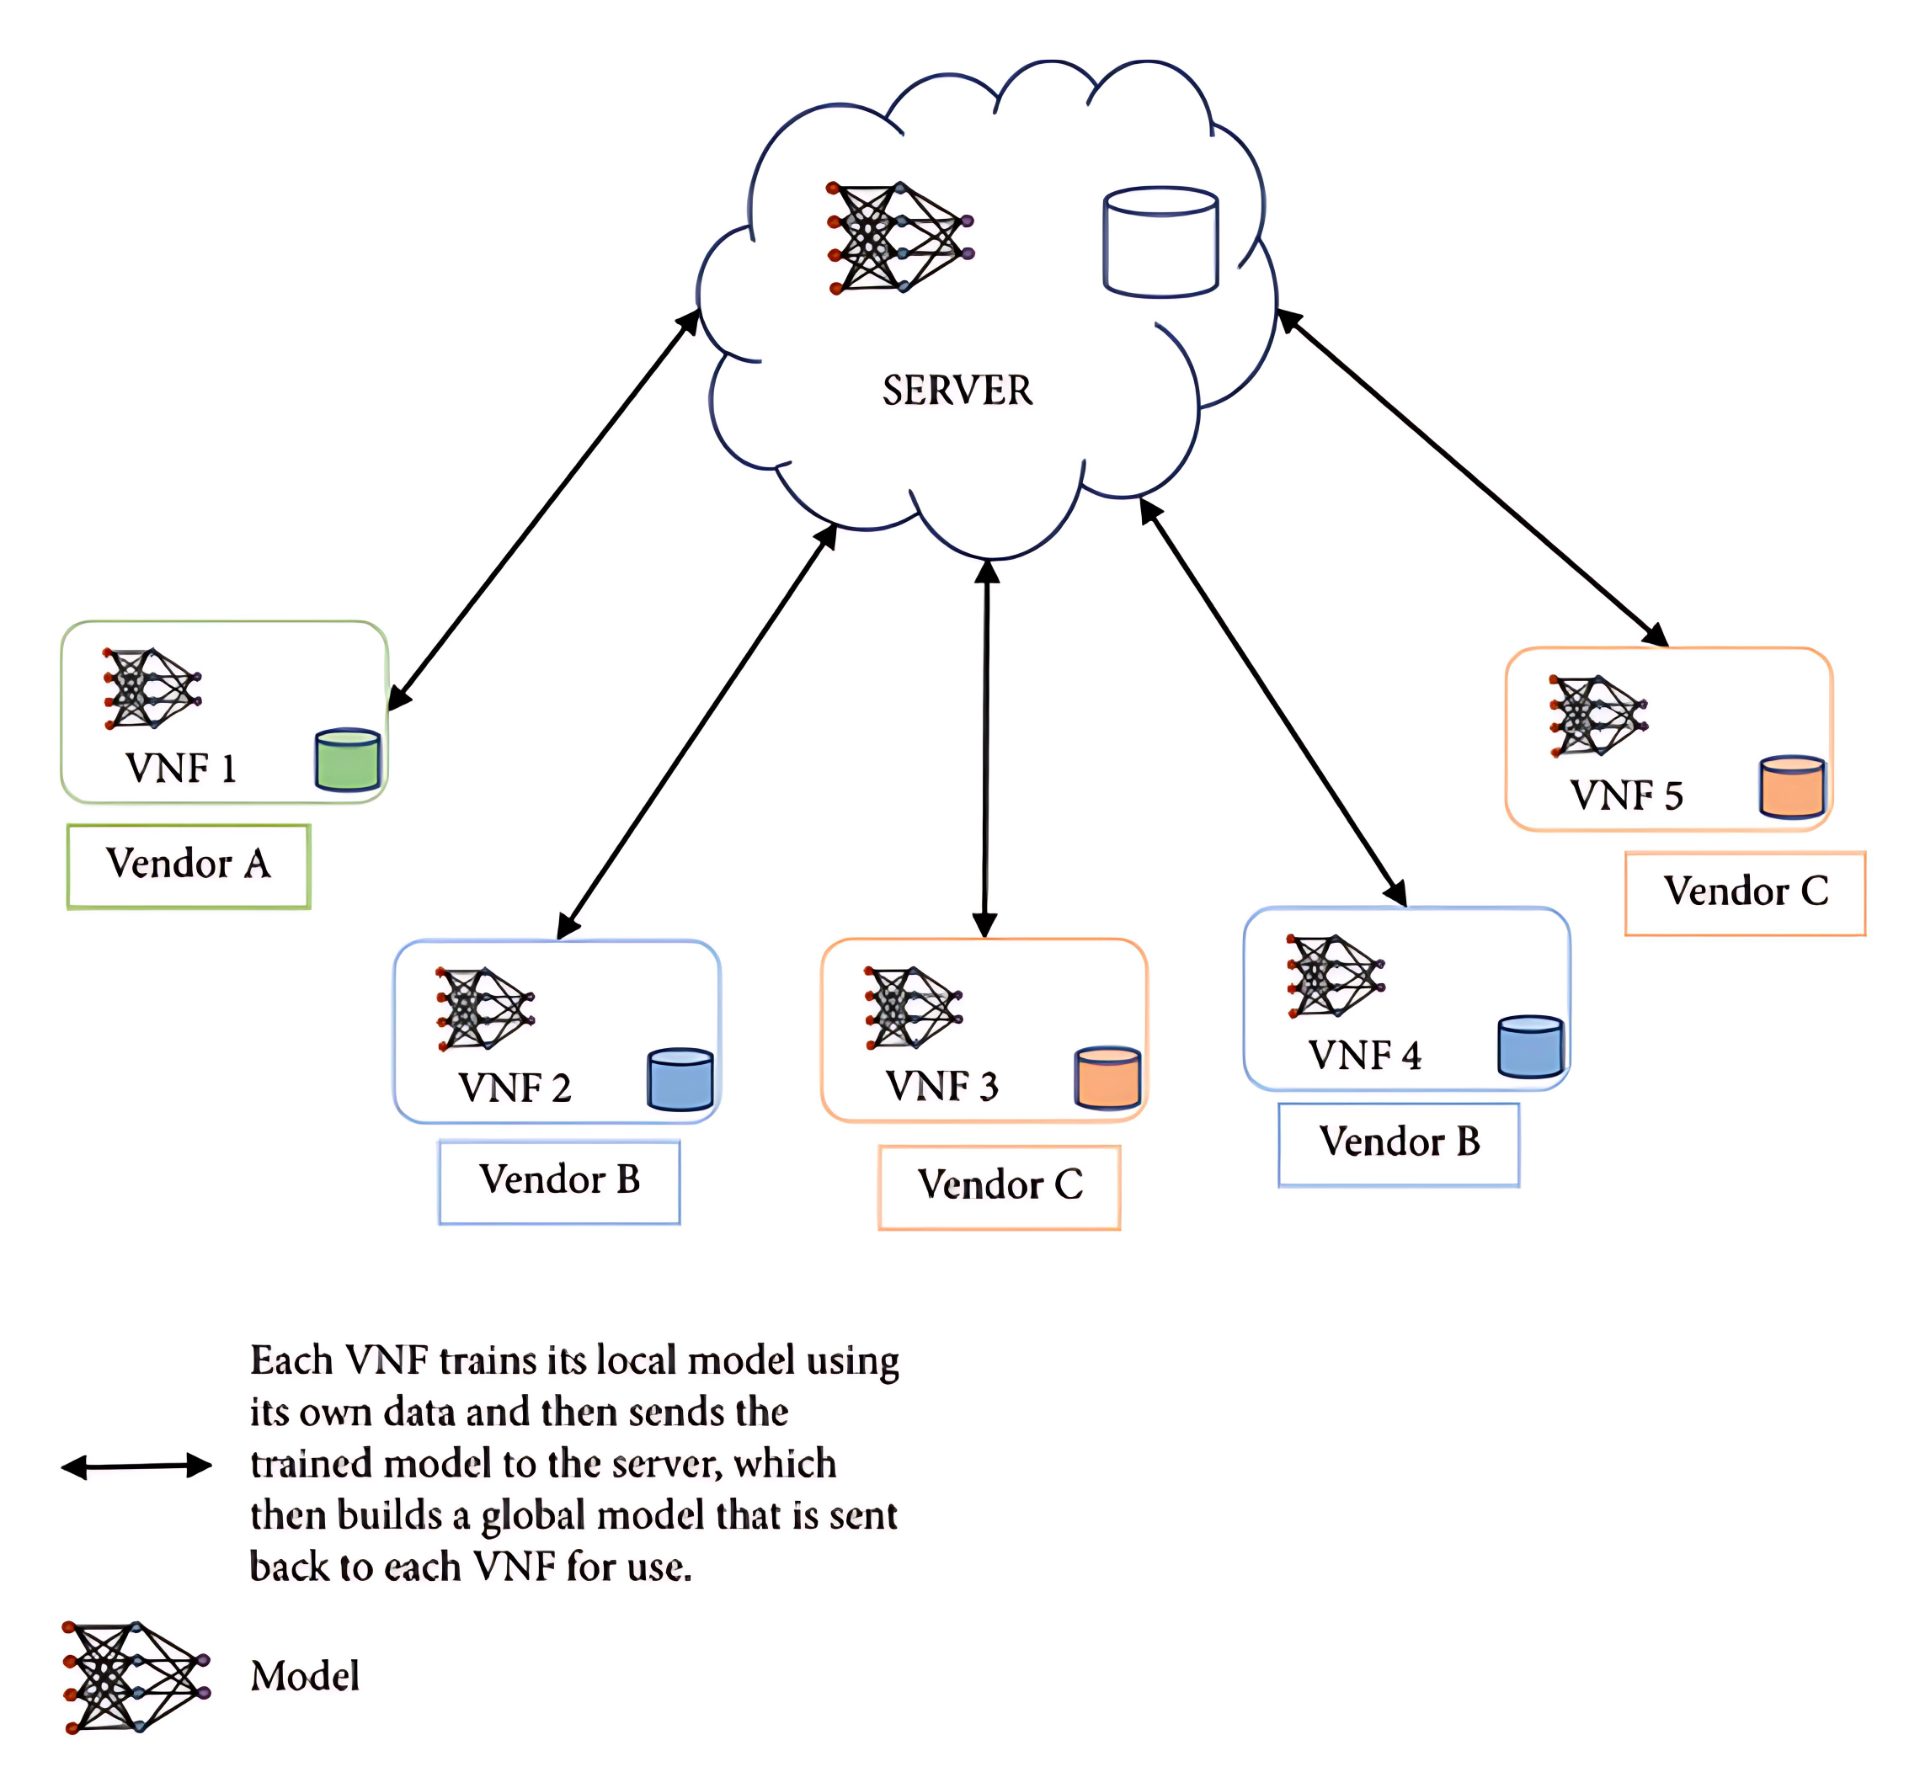
\includegraphics[width=0.85\textwidth]{./Figures/fig3.png}
    \caption{Figure 3 illustrates the architecture diversity across clients, showing how each local model (Virtual Network Function ) feeds into the broader federated learning system while maintaining autonomy over its training process.}
    \label{fig:local_models}
\end{figure}

\subsection{Stacking Ensemble Strategy}
\label{sec:stacking_ensemble_strategy}

Conventional federated learning (FL) methods like FedAvg assume that all clients use the same model architecture and share the same label space. However, this is rarely the case in real-world healthcare environments. To overcome these limitations, the proposed MStacking framework adopts a stacking ensemble strategy, which aggregates predictions instead of model parameters—making it flexible to both label and architectural heterogeneity.

The ensemble works in two levels (see Figure~\ref{fig:stacking_strategy}):

\begin{itemize}
    \item \textbf{Level-0 (Base Learners)}: Each client trains a binary classifier—such as a Random Forest (RF), Feedforward Neural Network (FNN), or Convolutional Neural Network (CNN)—on its local dataset. These models output probabilistic predictions for the normal class and one abnormal class.
    
    \item \textbf{Level-1 (Meta-Learner)}: A central model on the server aggregates predictions and density estimates (from Gaussian Mixture Models) sent by each client. It learns how to combine these varied outputs into a global multi-class classifier.
\end{itemize}

To enhance the quality of aggregation, each client also estimates the probability distribution of its input features and flags the classes it can recognize. These values are used to compute ensemble weights, which determine how much each client contributes to the final model.

As shown in Figure~\ref{fig:stacking_strategy}, this two-level stacking framework enables robust, privacy-preserving learning—even when clients have partial data or different computational capabilities.

\begin{figure}[h]
    \centering
    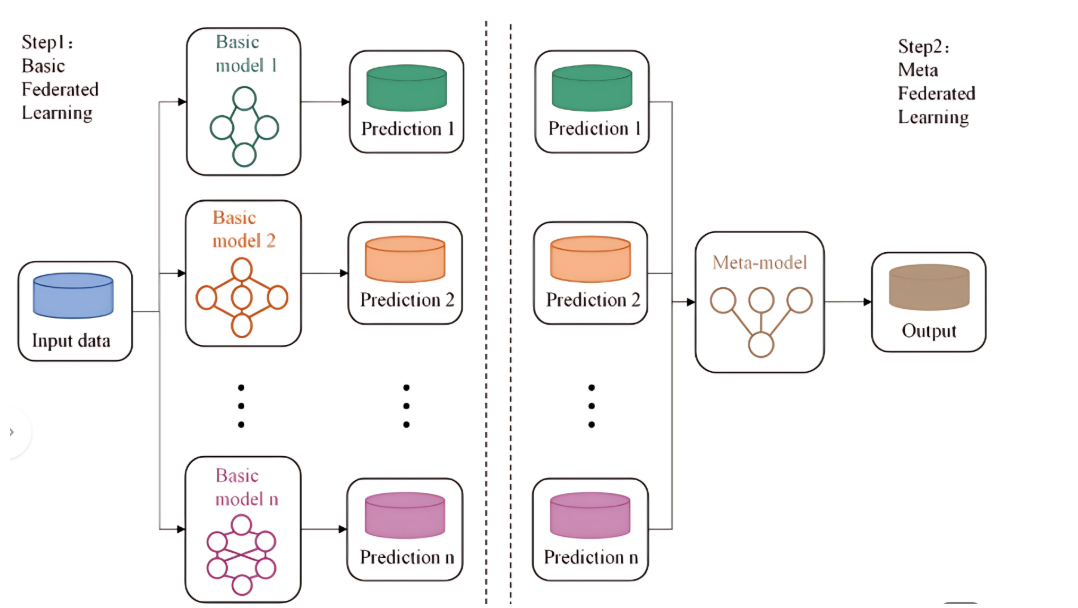
\includegraphics[width=0.85\textwidth]{./Figures/fig4.png}
    \caption{MStacking Two-Level Ensemble Architecture: Client-level models generate predictions and densities, aggregated by a central meta-learner into a global classifier.}
    \label{fig:stacking_strategy}
\end{figure}

\subsection{Federated Aggregation Process}
\label{sec:federated_aggregation}

Unlike traditional FL methods like FedAvg that rely on aggregating model parameters from identical architectures, MStacking takes a different route. It performs meta-level fusion, where predictions and feature distributions from each client’s model are combined at the server level.

Each participating client sends the following metadata to the central server:
\begin{itemize}
    \item Prediction probabilities from its trained binary classifier (e.g., RF, FNN, CNN).
    \item Density estimates of its local input data, modeled using Gaussian Mixture Models (GMMs).
    \item Class availability indicators that specify which classes the client has in its local dataset.
\end{itemize}

Using this information, the server constructs a global multi-class classifier $c_m(\theta)$ through a weighted integration of the client models. The weight $\omega_{j,m}$ assigned to client $j$ for class $m$ depends on:
\begin{itemize}
    \item Whether the class $m$ is present in client $j$’s data.
    \item The estimated quality of the local model, which factors in data distribution $f_{x_j}$ and the proportion of training samples from that client.
\end{itemize}

This aggregation strategy enables:
\begin{itemize}
    \item \textbf{Missing label handling}: Clients that lack some class labels can still contribute to the global model through inferred relationships.
    \item \textbf{Model flexibility}: Clients can use any architecture; uniformity is not required.
    \item \textbf{Privacy preservation}: Only high-level summaries (e.g., predictions and densities) are shared—never raw data or internal parameters.
\end{itemize}

\subsection{Evaluation Strategy}
\label{sec:evaluation_strategy}

To assess the performance and applicability of the MStacking framework, a structured evaluation plan will be followed using real-world and simulated data.

\textbf{Datasets:}
\begin{itemize}
    \item \textit{PhysioNet/CinC Challenge 2016}~\cite{clifford2016classification}: A large, annotated dataset of heart sounds, covering both normal and abnormal cases.
    \item \textit{Additional open-access PCG datasets}~\cite{liu2016open}: Used to simulate client-specific data distributions and class imbalances.
\end{itemize}

\textbf{Simulation Setup:}
\begin{itemize}
    \item Experiments will use Flower or FedML to simulate a federated environment.
    \item Clients will receive non-IID partitions, each containing the normal class and one abnormal class to replicate real-world heterogeneity.
\end{itemize}

\textbf{Metrics for Evaluation:}
\begin{itemize}
    \item Accuracy, Precision, Recall, F1-score (macro \& class-wise)
    \item AUROC for threshold robustness
    \item Confusion matrices to analyze prediction patterns
    \item Training time and communication cost for efficiency
    \item SHAP or similar methods for interpretability (if feasible)
\end{itemize}

\textbf{Baselines for Comparison:}
\begin{itemize}
    \item Centralized CNN trained on full data
    \item Traditional FedAvg with homogeneous models and labels
    \item Personalized FL with clustering or fine-tuning
\end{itemize}

\subsection{Implementation Details}
\label{sec:implementation}

\textbf{Development Environment:}
\begin{itemize}
    \item \textit{Language}: Python 3.x
    \item \textit{Federated Simulation}: Flower or FedML
    \item \textit{Deep Learning}: PyTorch
    \item \textit{Signal Processing}: OpenSMILE, LibROSA, and Continuous Wavelet Transform (CWT)
\end{itemize}

\textbf{Model Training:}
\begin{itemize}
    \item \textit{Optimizer}: Adam
    \item \textit{Monitoring}: Early stopping and validation tracking
    \item \textit{Architectures}: RF, FNN, CNN—based on local data modalities
\end{itemize}

\textbf{Execution Platform:}
\begin{itemize}
    \item \textit{Hardware}: Lab PCs or cloud-based GPUs (e.g., Google Colab, Kaggle)
    \item \textit{Version Control}: Git and GitHub
    \item \textit{Visualization \& Reporting}: Matplotlib, Seaborn, and LaTeX (Overleaf)
\end{itemize}

This implementation plan ensures that MStacking remains reproducible, scalable, and practical within an academic setting.

\chapter{Evaluation}


\section{Evaluation Objectives}
\label{sec:evaluation_objectives}

The evaluation phase aims to rigorously assess how well the proposed MStacking framework performs under realistic, decentralized healthcare scenarios. Key goals include:

\begin{itemize}
    \item Measuring the classification accuracy of the global multi-class model built via stacking.
    \item Comparing MStacking’s performance to traditional centralized learning and standard FL methods like FedAvg.
    \item Testing robustness against client heterogeneity, label misalignment, and imbalanced data distributions.
    \item Assessing system efficiency by tracking communication overhead and computational cost.
    \item Exploring the interpretability of predictions using feature attribution tools such as SHAP.
\end{itemize}

\section{Evaluation Metrics}
\label{sec:evaluation_metrics}

To ensure a comprehensive analysis, the following metrics will be employed:

\begin{itemize}
    \item \textbf{Accuracy}: Overall rate of correct predictions.
    \item \textbf{Precision, Recall, F1-Score}: Evaluated per class to reflect detection sensitivity and specificity. Macro-averaged versions will be emphasized to address class imbalance.
    \item \textbf{AUROC}: Measures the model's ability to distinguish between classes under varying thresholds.
    \item \textbf{Confusion Matrix}: Highlights where and how often misclassifications occur.
    \item \textbf{Model Communication Cost}: Total size of metadata exchanged between clients and the server.
    \item \textbf{Training Time per Round}: Gauges the runtime efficiency of global model updates.
    \item \textbf{Model Interpretability}: Investigated via SHAP or similar techniques to understand decision rationale.
\end{itemize}

\section{Experimental Setup}
\label{sec:experimental_setup}

\textbf{Datasets:}
\begin{itemize}
    \item \textit{PhysioNet/CinC Challenge 2016}~\cite{clifford2016classification}: Main benchmark dataset, with 3,000+ annotated heart sound recordings.
    \item \textit{Additional PCG datasets}~\cite{liu2016open}: Used to simulate diverse client data conditions and class variety.
\end{itemize}

\textbf{Client Configuration:}
\begin{itemize}
    \item 5 to 10 virtual clients will be created.
    \item Each client will have a non-IID data partition containing the normal class and a distinct abnormal class (star-structure).
    \item Clients will use varying model types (e.g., RF, FNN, CNN) to simulate hardware and algorithmic diversity.
\end{itemize}

\textbf{Baselines for Comparison:}
\begin{itemize}
    \item Centralized CNN trained on full data.
    \item Traditional FL (FedAvg) with uniform models and aligned labels.
    \item Personalized FL using clustered or fine-tuned models.
    \item Ablation Study to evaluate the role of metadata: predictions only vs. predictions + densities.
\end{itemize}

\section{Evaluation Procedure}
\label{sec:evaluation_procedure}

\textbf{1. Training Phase:}
\begin{itemize}
    \item Clients train local binary classifiers.
    \item Output includes prediction probabilities and Gaussian Mixture-based density estimates.
    \item These are sent to the server and integrated into a global model using stacking.
\end{itemize}

\textbf{2. Validation Phase:}
\begin{itemize}
    \item A held-out multi-class dataset is used to evaluate the global model.
    \item Metrics are updated after each training round.
\end{itemize}

\textbf{3. Stress Testing:}
\begin{itemize}
    \item Client dropouts to test resilience.
    \item Label noise to assess robustness.
    \item Imbalanced class samples to evaluate fairness.
\end{itemize}

\textbf{4. Result Analysis:}
\begin{itemize}
    \item Results will be visualized using ROC curves, training/validation loss plots, and confusion matrices.
    \item Comparative tables will summarize performance against baselines.
    \item A detailed discussion will highlight the strengths and trade-offs of MStacking.
\end{itemize}

\begin{table}[h]
\centering
\caption{Performance Comparison with Existing Methods}
\label{tab:performance_comparison}
\renewcommand{\arraystretch}{1.2}
\begin{tabular}{|p{2cm}|p{1cm}|p{1.5cm}|p{1.5cm}|p{1.5cm}|p{1.5cm}|p{2cm}|p{2cm}|}
\hline
\textbf{Method} & \textbf{Model Type} & \textbf{Setting} & \textbf{Data Mode} & \textbf{Accuracy} & \textbf{UF1 Score} & \textbf{UAR Score} & \textbf{Notes} \\ \hline
Centralized CNN & CNN & Centralized & Balanced & Moderate & Moderate & Moderate & Traditional learning with full label sharing \\ \hline
Fed-BIDS~\cite{fedbids2022} & RF + NN Meta & Federated & Balanced & High & Moderate & Moderate & Blends metadata for intrusion detection \\ \hline
Fed-MStacking (Homog.) & RF / FNN / CNN & Federated & Balanced & Higher & Higher & Higher & Uses identical architectures across clients \\ \hline
Fed-MStacking (Hetero) & RF + FNN + CNN & Federated & Balanced & Highest & Highest & Highest & Supports diverse models \& misaligned class labels (This work) \\ \hline
\end{tabular}
\end{table}

\chapter {Project Plan}
% \chapter{Evaluation}
\section{Work Breakdown Structure (WBS)}
To ensure smooth progress and timely delivery, the development of the MStacking framework is organized into seven structured phases. Each phase includes specific tasks that align with the overall project objectives:

\begin{table}[htbp]
\centering
\caption{Project Workflow Phases}
\label{tab:workflow}
\renewcommand{\arraystretch}{1.5} % Adjusted row spacing
\setlength{\tabcolsep}{6pt} % Increased horizontal padding
\begin{tabular}{|>{\bfseries}l!{\vrule width 1.2pt}p{9.5cm}|}
\hline
\rowcolor{gray!15}
\textbf{Phase} & \textbf{Description} \\ \hline

1. Research \& Literature Review & 
Study recent work in federated learning, stacking, heart sound classification, and AI in healthcare. \\ \hline

2. System Design & 
\vspace{-4mm}\begin{itemize}[leftmargin=*,nosep]
\item Define the MStacking architecture.
\item Plan client-server interactions and simulation topology.
\item Outline metadata and communication protocol.
\end{itemize} \\ \hline

3. Data Preparation & 
\vspace{-4mm}\begin{itemize}[leftmargin=*,nosep]
\item Preprocess PCG signals using MFCC and CWT.
\item Partition datasets into star-structured splits for FL simulation.
\item Validate multimodal input formats.
\end{itemize} \\ \hline

4. Local Model Implementation & 
\vspace{-4mm}\begin{itemize}[leftmargin=*,nosep]
\item Implement and train Random Forest, FNN, and CNN models.
\item Optimize each for local client data characteristics.
\end{itemize} \\ \hline

5. Stacking \& Federated Aggregation & 
\vspace{-4mm}\begin{itemize}[leftmargin=*,nosep]
\item Design metadata schema (predictions, densities).
\item Build meta-learner.
\item Integrate client outputs into a unified global model.
\end{itemize} \\ \hline

6. Evaluation \& Validation & 
\vspace{-4mm}\begin{itemize}[leftmargin=*,nosep]
\item Run experiments under non-IID, imbalanced, and noisy data scenarios.
\item Compare with centralized and traditional FL models.
\item Use metrics like accuracy, F1-score, AUROC, SHAP.
\end{itemize} \\ \hline

7. Documentation \& Presentation & 
\vspace{-4mm}\begin{itemize}[leftmargin=*,nosep]
\item Prepare final report, figures, and codebase documentation.
\item Present results and insights clearly for academic submission.
\end{itemize} \\ \hline
\end{tabular}
\end{table}

\begin{itemize}[leftmargin=*]
\item \textbf{Timeline:} Each phase is allocated 2-3 weeks with overlapping activities where possible
\item \textbf{Dependencies:} Sequential flow with iterative refinement loops between phases
\item \textbf{Deliverables:} Technical reports, prototype implementations, and evaluation results at each phase
\end{itemize}


\section{Timeline and Gantt Chart}
The project will be completed over a  four-month period, with major deliverables planned at each stage. Below  is the proposed timeline in a Gantt chart format:

\begin{figure}[htbp]
\centering
\begin{ganttchart}[
    % Chart configuration
    x unit=0.8cm,
    y unit title=0.8cm,
    y unit chart=0.8cm,
    vgrid,
    hgrid,
    title height=1,
    title label font=\bfseries\footnotesize,
    bar/.append style={fill=blue!30, rounded corners=2pt},
    bar height=0.6,
    bar label font=\footnotesize,
    milestone/.append style={fill=red!50, rounded corners=2pt},
    milestone label font=\footnotesize,
    group/.append style={draw=black, fill=green!20},
    group left shift=0,
    group right shift=0,
    group height=.3,
    group peaks tip position=0,
    bar incomplete/.append style={fill=yellow!30}
]{1}{16} % 16 weeks total
    
    % Months
    \gantttitle{July}{4}
    \gantttitle{August}{4}
    \gantttitle{September}{4}
    \gantttitle{October}{4} \\
    
    % Week numbers
    \gantttitlelist{1,...,16}{1} \\
    
    % Tasks
    \ganttbar{Literature Review \& Planning}{1}{5} \\
    \ganttbar{System Design}{1}{7} \\
    \ganttbar{Dataset Preparation}{5}{6} \\
    \ganttbar{Local Model Development}{5}{6} \\
    \ganttbar{Stacking \& Aggregation Module}{7}{12} \\
    \ganttbar{Evaluation \& Testing}{12}{14} \\
    \ganttbar{Documentation \& Final Report}{13}{16} \\
    \ganttbar{Presentation Preparation}{15}{16}
    
    % Vertical lines separating months
    \ganttvrule{4}{4}
    \ganttvrule{8}{8}
    \ganttvrule{12}{12}
\end{ganttchart}
\caption{Project Timeline Gantt Chart}
\label{fig:gantt}
\end{figure}

\section{Resources and Tools}
To develop, test,  and evaluate the MStacking framework efficiently, the following tools and platforms will be utilized:

\begin{itemize}[leftmargin=*]
\item \textbf{Software Tools:} Python 3.x, PyTorch, OpenSMILE, LibROSA, Flower, FedML, and Jupyter  Notebooks.
\item \textbf{Hardware:} University-provided GPU-enabled machines and cloud services like Google Colab and Kaggle  for additional compute support.
\item \textbf{Version Control:} Git and GitHub for collaborative development and version tracking.
\item \textbf{Documentation} Overleaf (LaTeX) for professional academic writing and formatting.
\item \textbf{Visualization Monitoring:} Matplotlib, Seaborn, and TensorBoard for experiment tracking and performance visualization.
\end{itemize}




\section{Risk Management}
Identified risks and corresponding mitigation strategies are outlined in the table below:
\begin{table}[htbp]
\centering
\caption{Risk and Mitigation Strategy}
\label{tab:workflow}
\renewcommand{\arraystretch}{1.3} % Adjusted row spacing
\setlength{\tabcolsep}{6pt} % Increased horizontal padding
\begin{tabular}{|<{\bfseries}l!{\vrule width 0.8pt}p{7.5cm}|}
\hline
\rowcolor{gray!15}
\textbf{Risk} & \textbf{Mitigation Strategy} \\ \hline

1. Insufficient compute resources & 
Leverage cloud-based platforms (Google Colab, Kaggle) for GPU access. \\ \hline

2. Time constraints during academic semester & 
Apply agile development cycles; prioritize the core MStacking framework before add-ons. \\ \hline

3. Lack of access to real-time medical data & 
Use realistic, publicly available datasets like PhysioNet to simulate clinical settings. \\ \hline

4. Debugging federated heterogeneity issues & 
Conduct isolated tests for each local model type (RF, FNN, CNN) before integration. \\ \hline


\end{tabular}
\end{table}




\bibliographystyle{plain}
\bibliography{references}


% \bibliographystyle{IEEEtran}  % or plain, apalike, etc.
% \bibliography{myreferences}  % your .bib file name without extension


% \bibliographystyle{plainnat}
% \bibliography{references}  % this uses references.bib



\end{document}